% Options for packages loaded elsewhere
\PassOptionsToPackage{unicode}{hyperref}
\PassOptionsToPackage{hyphens}{url}
%
\documentclass[
  11pt,
]{article}
\usepackage{amsmath,amssymb}
\usepackage{iftex}
\ifPDFTeX
  \usepackage[T1]{fontenc}
  \usepackage[utf8]{inputenc}
  \usepackage{textcomp} % provide euro and other symbols
\else % if luatex or xetex
  \usepackage{unicode-math} % this also loads fontspec
  \defaultfontfeatures{Scale=MatchLowercase}
  \defaultfontfeatures[\rmfamily]{Ligatures=TeX,Scale=1}
\fi
\usepackage{lmodern}
\ifPDFTeX\else
  % xetex/luatex font selection
\fi
% Use upquote if available, for straight quotes in verbatim environments
\IfFileExists{upquote.sty}{\usepackage{upquote}}{}
\IfFileExists{microtype.sty}{% use microtype if available
  \usepackage[]{microtype}
  \UseMicrotypeSet[protrusion]{basicmath} % disable protrusion for tt fonts
}{}
\makeatletter
\@ifundefined{KOMAClassName}{% if non-KOMA class
  \IfFileExists{parskip.sty}{%
    \usepackage{parskip}
  }{% else
    \setlength{\parindent}{0pt}
    \setlength{\parskip}{6pt plus 2pt minus 1pt}}
}{% if KOMA class
  \KOMAoptions{parskip=half}}
\makeatother
\usepackage{xcolor}
\usepackage[margin=1in]{geometry}
\usepackage{color}
\usepackage{fancyvrb}
\newcommand{\VerbBar}{|}
\newcommand{\VERB}{\Verb[commandchars=\\\{\}]}
\DefineVerbatimEnvironment{Highlighting}{Verbatim}{commandchars=\\\{\}}
% Add ',fontsize=\small' for more characters per line
\usepackage{framed}
\definecolor{shadecolor}{RGB}{248,248,248}
\newenvironment{Shaded}{\begin{snugshade}}{\end{snugshade}}
\newcommand{\AlertTok}[1]{\textcolor[rgb]{0.94,0.16,0.16}{#1}}
\newcommand{\AnnotationTok}[1]{\textcolor[rgb]{0.56,0.35,0.01}{\textbf{\textit{#1}}}}
\newcommand{\AttributeTok}[1]{\textcolor[rgb]{0.13,0.29,0.53}{#1}}
\newcommand{\BaseNTok}[1]{\textcolor[rgb]{0.00,0.00,0.81}{#1}}
\newcommand{\BuiltInTok}[1]{#1}
\newcommand{\CharTok}[1]{\textcolor[rgb]{0.31,0.60,0.02}{#1}}
\newcommand{\CommentTok}[1]{\textcolor[rgb]{0.56,0.35,0.01}{\textit{#1}}}
\newcommand{\CommentVarTok}[1]{\textcolor[rgb]{0.56,0.35,0.01}{\textbf{\textit{#1}}}}
\newcommand{\ConstantTok}[1]{\textcolor[rgb]{0.56,0.35,0.01}{#1}}
\newcommand{\ControlFlowTok}[1]{\textcolor[rgb]{0.13,0.29,0.53}{\textbf{#1}}}
\newcommand{\DataTypeTok}[1]{\textcolor[rgb]{0.13,0.29,0.53}{#1}}
\newcommand{\DecValTok}[1]{\textcolor[rgb]{0.00,0.00,0.81}{#1}}
\newcommand{\DocumentationTok}[1]{\textcolor[rgb]{0.56,0.35,0.01}{\textbf{\textit{#1}}}}
\newcommand{\ErrorTok}[1]{\textcolor[rgb]{0.64,0.00,0.00}{\textbf{#1}}}
\newcommand{\ExtensionTok}[1]{#1}
\newcommand{\FloatTok}[1]{\textcolor[rgb]{0.00,0.00,0.81}{#1}}
\newcommand{\FunctionTok}[1]{\textcolor[rgb]{0.13,0.29,0.53}{\textbf{#1}}}
\newcommand{\ImportTok}[1]{#1}
\newcommand{\InformationTok}[1]{\textcolor[rgb]{0.56,0.35,0.01}{\textbf{\textit{#1}}}}
\newcommand{\KeywordTok}[1]{\textcolor[rgb]{0.13,0.29,0.53}{\textbf{#1}}}
\newcommand{\NormalTok}[1]{#1}
\newcommand{\OperatorTok}[1]{\textcolor[rgb]{0.81,0.36,0.00}{\textbf{#1}}}
\newcommand{\OtherTok}[1]{\textcolor[rgb]{0.56,0.35,0.01}{#1}}
\newcommand{\PreprocessorTok}[1]{\textcolor[rgb]{0.56,0.35,0.01}{\textit{#1}}}
\newcommand{\RegionMarkerTok}[1]{#1}
\newcommand{\SpecialCharTok}[1]{\textcolor[rgb]{0.81,0.36,0.00}{\textbf{#1}}}
\newcommand{\SpecialStringTok}[1]{\textcolor[rgb]{0.31,0.60,0.02}{#1}}
\newcommand{\StringTok}[1]{\textcolor[rgb]{0.31,0.60,0.02}{#1}}
\newcommand{\VariableTok}[1]{\textcolor[rgb]{0.00,0.00,0.00}{#1}}
\newcommand{\VerbatimStringTok}[1]{\textcolor[rgb]{0.31,0.60,0.02}{#1}}
\newcommand{\WarningTok}[1]{\textcolor[rgb]{0.56,0.35,0.01}{\textbf{\textit{#1}}}}
\usepackage{graphicx}
\makeatletter
\def\maxwidth{\ifdim\Gin@nat@width>\linewidth\linewidth\else\Gin@nat@width\fi}
\def\maxheight{\ifdim\Gin@nat@height>\textheight\textheight\else\Gin@nat@height\fi}
\makeatother
% Scale images if necessary, so that they will not overflow the page
% margins by default, and it is still possible to overwrite the defaults
% using explicit options in \includegraphics[width, height, ...]{}
\setkeys{Gin}{width=\maxwidth,height=\maxheight,keepaspectratio}
% Set default figure placement to htbp
\makeatletter
\def\fps@figure{htbp}
\makeatother
\setlength{\emergencystretch}{3em} % prevent overfull lines
\providecommand{\tightlist}{%
  \setlength{\itemsep}{0pt}\setlength{\parskip}{0pt}}
\setcounter{secnumdepth}{-\maxdimen} % remove section numbering
\ifLuaTeX
  \usepackage{selnolig}  % disable illegal ligatures
\fi
\usepackage{bookmark}
\IfFileExists{xurl.sty}{\usepackage{xurl}}{} % add URL line breaks if available
\urlstyle{same}
\hypersetup{
  pdftitle={Assignment 2 - Report},
  pdfauthor={Eleni Liarou, Zoë Azra Blei, Frederieke Loth, group 20},
  hidelinks,
  pdfcreator={LaTeX via pandoc}}

\title{Assignment 2 - Report}
\author{Eleni Liarou, Zoë Azra Blei, Frederieke Loth, group 20}
\date{2025-03-07}

\begin{document}
\maketitle

\section{Exercise 1: Titanic}\label{exercise-1-titanic}

\paragraph{Section a}\label{section-a}

\begin{verbatim}
##      Name           PClass         Age          Sex         Survived    
##  Length:1313        1st:322   Min.   : 0    female:462   Min.   :0.000  
##  Class :character   2nd:280   1st Qu.:21    male  :851   1st Qu.:0.000  
##  Mode  :character   3rd:711   Median :28                 Median :0.000  
##                               Mean   :30                 Mean   :0.343  
##                               3rd Qu.:39                 3rd Qu.:1.000  
##                               Max.   :71                 Max.   :1.000  
##                               NA's   :557
\end{verbatim}

From the summary, we see that 3rd class passengers outnumbered those in
1st and 2nd classes combined. 35\% of passengers were female, and 65\%
male. Half the passengers were aged between 21 and 39, with 557 missing
age values. The survival rate has a mean of 0.3427, indicating around
one-third of passengers survived. However, the dataset is incomplete,
containing data for only 1,313 of the 2,224 passengers.

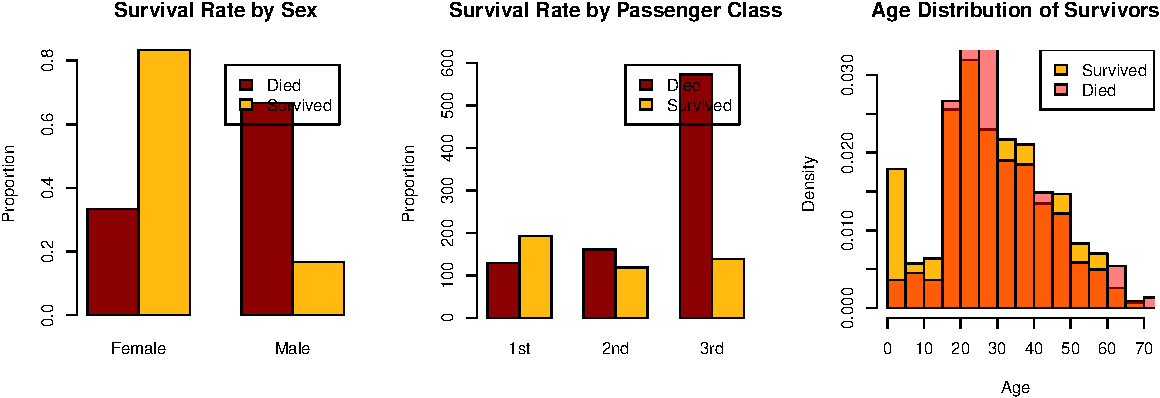
\includegraphics{ReportAssignment2_files/figure-latex/unnamed-chunk-2-1.pdf}

More males than females died, and most 3rd class passengers did not
survive. The highest number of both survivors and deaths were among
passengers aged 20 to 30.

From the below graphs we see that the majority of passengers were around
25 years old, with fewer individuals in older age groups. 1st class
passengers were generally older than those in 2nd and 3rd class.

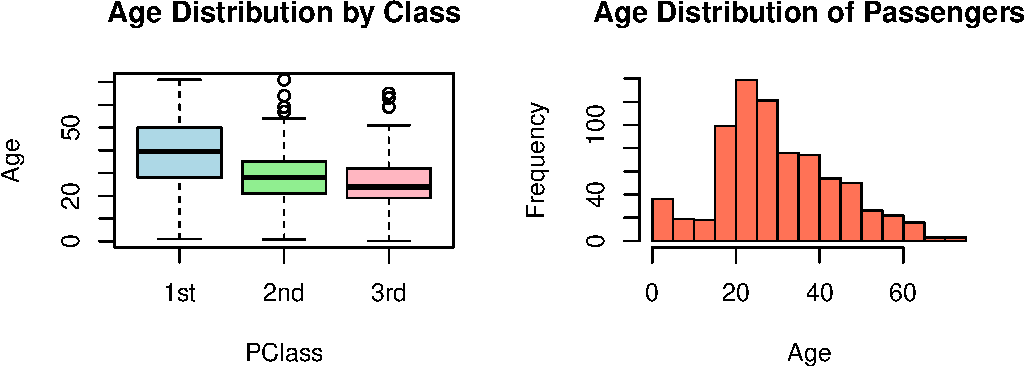
\includegraphics{ReportAssignment2_files/figure-latex/unnamed-chunk-3-1.pdf}

Let's examine how the sexes were distributed over the passenger classes.

\begin{Shaded}
\begin{Highlighting}[]
\NormalTok{sex\_class }\OtherTok{\textless{}{-}}\FunctionTok{xtabs}\NormalTok{(}\SpecialCharTok{\textasciitilde{}}\NormalTok{PClass}\SpecialCharTok{+}\NormalTok{Sex, }\AttributeTok{data=}\NormalTok{data\_titanic)}
\NormalTok{sex\_class}
\end{Highlighting}
\end{Shaded}

\begin{verbatim}
##       Sex
## PClass female male
##    1st    143  179
##    2nd    107  173
##    3rd    212  499
\end{verbatim}

As expected, since there are more males overall, each passenger class
has a higher number of males.

\begin{Shaded}
\begin{Highlighting}[]
\NormalTok{sex\_class\_surv }\OtherTok{\textless{}{-}} \FunctionTok{xtabs}\NormalTok{(Survived}\SpecialCharTok{\textasciitilde{}}\NormalTok{PClass}\SpecialCharTok{+}\NormalTok{Sex, }\AttributeTok{data=}\NormalTok{data\_titanic)}
\FunctionTok{round}\NormalTok{(sex\_class\_surv}\SpecialCharTok{/}\NormalTok{sex\_class, }\DecValTok{2}\NormalTok{)}
\end{Highlighting}
\end{Shaded}

\begin{verbatim}
##       Sex
## PClass female male
##    1st   0.94 0.33
##    2nd   0.88 0.14
##    3rd   0.38 0.12
\end{verbatim}

The survival rate decreases from 1st to 3rd class, but remains
significantly higher for females across all classes. However, the
difference in survival between females and males is less pronounced in
3rd class.

We will now fit a logistic regression model to investigate the
association between the survival status and the
predictors~\emph{PClass},~\emph{Age}~and~\emph{Sex.}

\begin{Shaded}
\begin{Highlighting}[]
\NormalTok{add\_mod }\OtherTok{\textless{}{-}} \FunctionTok{glm}\NormalTok{(Survived }\SpecialCharTok{\textasciitilde{}}\NormalTok{ PClass }\SpecialCharTok{+}\NormalTok{ Age }\SpecialCharTok{+}\NormalTok{ Sex, }\AttributeTok{data =}\NormalTok{ titanic\_clean, }\AttributeTok{family =}\NormalTok{ binomial)}
\FunctionTok{summary}\NormalTok{(add\_mod)}\SpecialCharTok{$}\NormalTok{coefficients}
\end{Highlighting}
\end{Shaded}

\begin{verbatim}
##             Estimate Std. Error z value Pr(>|z|)
## (Intercept)   3.7597    0.39757    9.46 3.18e-21
## PClass2nd    -1.2920    0.26008   -4.97 6.78e-07
## PClass3rd    -2.5214    0.27666   -9.11 7.95e-20
## Age          -0.0392    0.00762   -5.14 2.69e-07
## Sexmale      -2.6314    0.20151  -13.06 5.68e-39
\end{verbatim}

\begin{Shaded}
\begin{Highlighting}[]
\FunctionTok{cat}\NormalTok{(}\StringTok{"AIC:"}\NormalTok{, }\FunctionTok{AIC}\NormalTok{(add\_mod))}
\end{Highlighting}
\end{Shaded}

\begin{verbatim}
## AIC: 705
\end{verbatim}

The odds can be calculated using the estimates of the above table as:

\[
\text{odds} = e^{\text{log-odds}} = e^{3.7597 + (-1.292) \times \text{PClass2nd} + (-2.521) \times \text{PClass3rd} + (-0.0392) \times \text{Age} + (-2.631) \times \text{Sexmale}} 
\]

Being in 2nd or 3rd class significantly reduces the probability of
survival compared to 1st class. Older age is associated with a lower
likelihood of survival, while being male significantly decreases the
chances of survival compared to being female. The magnitude of the
coefficients reflects the sensitivity of survival odds to each variable.
Being male has the largest negative effect on survival, while age has
the smallest effect in comparison to class and sex.

\paragraph{Section b}\label{section-b}

Investigating the interaction between Age and PClass.

\begin{Shaded}
\begin{Highlighting}[]
\FunctionTok{summary}\NormalTok{(}\FunctionTok{glm}\NormalTok{(Survived}\SpecialCharTok{\textasciitilde{}}\NormalTok{Age}\SpecialCharTok{*}\NormalTok{PClass, }\AttributeTok{data=}\NormalTok{data\_titanic, }\AttributeTok{family=}\StringTok{"binomial"}\NormalTok{), }\AttributeTok{test=}\StringTok{"Chisq"}\NormalTok{)}\SpecialCharTok{$}\NormalTok{coefficients}
\end{Highlighting}
\end{Shaded}

\begin{verbatim}
##               Estimate Std. Error z value Pr(>|z|)
## (Intercept)    1.92298    0.43625   4.408 1.04e-05
## Age           -0.03584    0.00996  -3.600 3.18e-04
## PClass2nd     -0.74428    0.57155  -1.302 1.93e-01
## PClass3rd     -2.29007    0.54057  -4.236 2.27e-05
## Age:PClass2nd -0.01321    0.01587  -0.832 4.05e-01
## Age:PClass3rd  0.00464    0.01594   0.291 7.71e-01
\end{verbatim}

\begin{Shaded}
\begin{Highlighting}[]
\FunctionTok{cat}\NormalTok{(}\StringTok{"AIC:"}\NormalTok{, }\FunctionTok{AIC}\NormalTok{(}\FunctionTok{glm}\NormalTok{(Survived }\SpecialCharTok{\textasciitilde{}}\NormalTok{ Age }\SpecialCharTok{*}\NormalTok{ PClass, }\AttributeTok{data=}\NormalTok{data\_titanic, }\AttributeTok{family=}\StringTok{"binomial"}\NormalTok{)))}
\end{Highlighting}
\end{Shaded}

\begin{verbatim}
## AIC: 921
\end{verbatim}

We now investigate the interaction between Age and Sex.

\begin{Shaded}
\begin{Highlighting}[]
\FunctionTok{summary}\NormalTok{(}\FunctionTok{glm}\NormalTok{(Survived}\SpecialCharTok{\textasciitilde{}}\NormalTok{Age}\SpecialCharTok{*}\NormalTok{Sex, }\AttributeTok{data=}\NormalTok{data\_titanic, }\AttributeTok{family=}\StringTok{"binomial"}\NormalTok{), }\AttributeTok{test=}\StringTok{"Chisq"}\NormalTok{)}\SpecialCharTok{$}\NormalTok{coefficients}
\end{Highlighting}
\end{Shaded}

\begin{verbatim}
##             Estimate Std. Error z value Pr(>|z|)
## (Intercept)   0.3011     0.2990    1.01 3.14e-01
## Age           0.0294     0.0101    2.91 3.58e-03
## Sexmale      -0.5999     0.4080   -1.47 1.42e-01
## Age:Sexmale  -0.0657     0.0137   -4.80 1.57e-06
\end{verbatim}

\begin{Shaded}
\begin{Highlighting}[]
\FunctionTok{cat}\NormalTok{(}\StringTok{"AIC:"}\NormalTok{, }\FunctionTok{AIC}\NormalTok{(}\FunctionTok{glm}\NormalTok{(Survived }\SpecialCharTok{\textasciitilde{}}\NormalTok{ Age }\SpecialCharTok{*}\NormalTok{ Sex, }\AttributeTok{data=}\NormalTok{data\_titanic, }\AttributeTok{family=}\StringTok{"binomial"}\NormalTok{)))}
\end{Highlighting}
\end{Shaded}

\begin{verbatim}
## AIC: 779
\end{verbatim}

The interaction between Age and PClass does not have a significant
effect on survival. The p-values for both Age:PClass2nd (0.405) and
Age:PClass3rd (0.771) are greater than the 0.05 threshold, indicating
that these interaction terms should not be included in the final model.
The interaction between Age and Sex is statistically significant, with a
p-value of 1.57e-06 \textless{} 0.05 threshold. This suggests that the
relationship between Age and survival differs by Sex, and thus, the
interaction term should be included in the final model.

So the final model is:

\begin{Shaded}
\begin{Highlighting}[]
\NormalTok{final\_model }\OtherTok{\textless{}{-}} \FunctionTok{glm}\NormalTok{(Survived }\SpecialCharTok{\textasciitilde{}}\NormalTok{ PClass }\SpecialCharTok{+}\NormalTok{ Age}\SpecialCharTok{*}\NormalTok{Sex, }\AttributeTok{data=}\NormalTok{data\_titanic, }\AttributeTok{family=}\StringTok{"binomial"}\NormalTok{)}
\FunctionTok{summary}\NormalTok{(final\_model, }\AttributeTok{test=}\StringTok{"Chisq"}\NormalTok{)}\SpecialCharTok{$}\NormalTok{coefficients}
\end{Highlighting}
\end{Shaded}

\begin{verbatim}
##             Estimate Std. Error z value Pr(>|z|)
## (Intercept)  2.75656     0.4376   6.299 3.00e-10
## PClass2nd   -1.54337     0.2874  -5.371 7.83e-08
## PClass3rd   -2.65398     0.2914  -9.107 8.47e-20
## Age          0.00244     0.0114   0.214 8.30e-01
## Sexmale     -0.50819     0.4425  -1.148 2.51e-01
## Age:Sexmale -0.07559     0.0150  -5.036 4.74e-07
\end{verbatim}

\begin{Shaded}
\begin{Highlighting}[]
\FunctionTok{cat}\NormalTok{(}\StringTok{"AIC:"}\NormalTok{, }\FunctionTok{AIC}\NormalTok{(}\FunctionTok{glm}\NormalTok{(Survived }\SpecialCharTok{\textasciitilde{}}\NormalTok{ PClass }\SpecialCharTok{+}\NormalTok{ Age}\SpecialCharTok{*}\NormalTok{Sex, }\AttributeTok{data=}\NormalTok{data\_titanic, }\AttributeTok{family=}\StringTok{"binomial"}\NormalTok{)))}
\end{Highlighting}
\end{Shaded}

\begin{verbatim}
## AIC: 679
\end{verbatim}

This model has an AIC of 679, which is lower than the additive model's
AIC of 705. Since a lower AIC indicates a better balance between fit and
complexity, we choose this model over the additive one.

Using this model, we can now estimate the probability of survival for
each combination of levels of the factors PClass and~\emph{Sex}~for a
person of age 55.

\begin{Shaded}
\begin{Highlighting}[]
\NormalTok{new\_data }\OtherTok{\textless{}{-}} \FunctionTok{expand.grid}\NormalTok{(}\AttributeTok{Age =} \DecValTok{55}\NormalTok{, }\AttributeTok{PClass =} \FunctionTok{levels}\NormalTok{(data\_titanic}\SpecialCharTok{$}\NormalTok{PClass), }
                        \AttributeTok{Sex =} \FunctionTok{levels}\NormalTok{(data\_titanic}\SpecialCharTok{$}\NormalTok{Sex))}
\NormalTok{probabilities }\OtherTok{\textless{}{-}} \FunctionTok{predict}\NormalTok{(final\_model, }\AttributeTok{newdata =}\NormalTok{ new\_data, }\AttributeTok{type =} \StringTok{"response"}\NormalTok{)}
\FunctionTok{cbind}\NormalTok{(new\_data, }\AttributeTok{Survival\_Prob =} \FunctionTok{round}\NormalTok{(probabilities, }\DecValTok{3}\NormalTok{))}
\end{Highlighting}
\end{Shaded}

\begin{verbatim}
##   Age PClass    Sex Survival_Prob
## 1  55    1st female         0.947
## 2  55    2nd female         0.794
## 3  55    3rd female         0.559
## 4  55    1st   male         0.145
## 5  55    2nd   male         0.035
## 6  55    3rd   male         0.012
\end{verbatim}

From the table above, we see once again that being female significantly
increases the chance of survival, while survival probability decreases
progressively from 1st to 3rd class.

\paragraph{Section c}\label{section-c}

To predict survival status, we split the data into training (80\%) and
testing (20\%) subsets. We train a logistic regression model using glm()
on the training set and use predict() to generate survival probabilities
for the test set. After applying a threshold of 0.5 we classify
passengers as survived or not. The quality of the prediction can be
measured by accuracy (correct predictions/total cases) and other metrics
such as AUC-ROC and precision or recall, which provide a more detailed
evaluation, especially when dealing with class imbalance.

\paragraph{Section d}\label{section-d}

We will use Fisher's exact test to examine the effect of sex on survival
status since it is more suitable for 2x2 tables and the 2-test to
investigate the effect of class on survival status.

\begin{verbatim}
## 
##  Fisher's Exact Test for Count Data
## 
## data:  cont_table_sex
## p-value <2e-16
## alternative hypothesis: true odds ratio is not equal to 1
## 95 percent confidence interval:
##  0.0762 0.1316
## sample estimates:
## odds ratio 
##        0.1
\end{verbatim}

\begin{verbatim}
## We performed a 2-test to investigate the relationship between PClass and Survived.
\end{verbatim}

\begin{verbatim}
## Chi-squared value: 172 Degrees of freedom: 2 p-value: 3.85e-38
\end{verbatim}

Both tests show that class and sex are strongly associated with
survival.

The 2-test for the relationship between passenger class and survival
status reveals a significant association, with a test statistic of 172
and a p-value less than 2e-16. This indicates that survival is strongly
influenced by passenger class, with the null hypothesis of no
association being rejected. Similarly, Fisher's Exact Test for gender
and survival status shows a highly significant result (p-value
\textless{} 2e-16). The odds ratio of 0.1 suggests that females have
much higher odds of surviving than males, with a 95\% confidence
interval (0.0762, 0.1316) confirming that the true odds ratio is
significantly less than 1. This supports the conclusion that being
female substantially increases the chances of survival.

\paragraph{Section e}\label{section-e}

The approach in (d) is not wrong; it simply tests for associations
between categorical variables, whereas the approach in (a) and (b)
allows for adjustment of multiple factors and prediction of survival
probability.

\textbf{Logistic regression}

Advantages: Can handle both categorical and continuous predictors.
Provides odds ratios, making interpretation straightforward. Allows for
adjustment of multiple factors simultaneously. Can be used for
predicting survival probability.

Disadvantages: Assumes a linear relationship between predictor and
log-odds of the outcome. Can suffer from over-fitting if the sample size
is too small.

\textbf{2-Test}

Advantages: Simple and easy to compute even for large datasets. Works
well for categorical explanatory variables and can be applied to tables
larger than 2x2.

Disadvantages: Less accurate for small sample sizes (expected counts
\textless{} 5 can make results unreliable). Only tells you whether
dependence exists, not the nature of the dependency. Cannot be used for
prediction.

\textbf{Fisher Test}

same as the 2-test except for the following

Advantages: Accurate for small sample sizes. Provides exact p-value

Disadvantages: Can be used for tables larger than 2x2 but is
computationally expensive.

\section{Exercise 2: Military Coups}\label{exercise-2-military-coups}

\paragraph{Section a}\label{section-a-1}

\paragraph{Section b}\label{section-b-1}

\paragraph{Section c}\label{section-c-1}

\section{Exercise 3: Stormer
viscometer}\label{exercise-3-stormer-viscometer}

\paragraph{Section a}\label{section-a-2}

\paragraph{Section b}\label{section-b-2}

\paragraph{Section c}\label{section-c-2}

\paragraph{Section d}\label{section-d-1}

\paragraph{Section e}\label{section-e-1}

\end{document}
